 
%-------------------------------------------
% FILE:    training.tex
% AUTHOR:  Rachel Anderson
% DATE:    2012
%
% Master latex file for python training.
%
%-------------------------------------------


% Define style of document
\documentclass[12pt,letter]{book}% for A4 paper

% Include packages
\usepackage{graphicx,palatino,palatcm}
\usepackage{amsmath,amssymb,amsfonts} % Typical maths resource packages
\usepackage{graphics}                 % Packages to allow inclusion of graphics
\usepackage{caption,topcapt}
\usepackage{rotating}
\usepackage{natbib}
\usepackage{wrapfig}
\usepackage{apjfonts}
\usepackage{amssymb}
\usepackage{multicol}
\usepackage{color}
\usepackage[colorlinks=true, urlcolor=blue]{hyperref}
\DeclareGraphicsRule{.tif}{png}{.png}{`convert #1 `dirname #1`/`basename #1 .tif`.png}

% Set the page layout
\setlength{\parindent}{0mm}      %sangria
\setlength{\textwidth}{161mm}
\setlength{\topmargin}{0mm}
\setlength{\textheight}{210mm}
\setlength{\oddsidemargin}{5mm}
\setlength{\evensidemargin}{-\oddsidemargin}
\setlength{\parskip}{3mm}     %espacio entre paragraphs
\linespread{1.0}   %determina el espacio entre lineas 1.6 = doble espacio

\usepackage{fancyhdr}
\pagestyle{fancy}
\renewcommand{\chaptermark}[1]%
   {\markboth{\uppercase{\thechapter.\ #1}}{}}
\renewcommand{\sectionmark}[1]%
   {\markright{\uppercase{\thesection.\ #1}}}
\newcommand{\helv}{%
   \fontfamily{phv}\fontseries{b}\fontsize{9}{11}\selectfont}
\lhead[\helv \thepage]{\helv \rightmark}
\rhead[\helv \leftmark]{\helv \thepage}
\cfoot{}
\newcommand{\captionlabeldelim}{---}

\usepackage[Leonardo]{fncychap}

\ChNameVar{\fontsize{14}{16}\usefont{OT1}{phv}{m}{n}\selectfont} 
\ChNumVar{\fontsize{60}{62}\usefont{OT1}{ptm}{m}{n}\selectfont} 
\ChTitleVar{\Huge\bfseries\rm}
\ChRuleWidth{1pt} 
 

 
% Extra definitions
\renewcommand{\sectionmark}[1]{\markright{\thesection.\ #1}}
\renewcommand{\chaptermark}[1]{\markboth{Chapter   \thechapter.
    {#1}}{Chapter  \thechapter.  {#1}}}

\renewcommand{\captionfont}{\footnotesize}
\renewcommand{\captionlabelfont}{\small \sc}

\makeatletter
\newcommand\figcaption{\def\@captype{figure}\caption}
\newcommand\tabcaption{\def\@captype{table}\caption}
\makeatother
\makeindex

%I added these:

\newcommand{\pytab}{python> }
\newcommand{\termtab}{$\gg$ }
\newcommand{\pyraftab}{pyraf> }
\newcounter{exercise}
\setcounter{exercise}{1}
\usepackage{alltt}

%
\flushbottom
\setcounter{tocdepth}{2}

% Start of document
\begin{document}

\pagenumbering{arabic}
\title{Python Training}

\author{Rachel Anderson}

\addtocounter{page}{-2}
 
\begin{titlepage}
\rule{165mm}{0.8mm}
 Version 2.0 \\
 July 2014

\vspace{30mm}
{\Huge Basic PyRAF }

\vspace{80mm}

\begin{minipage}[l]{80mm}

\includegraphics[width=8cm]{logo.jpg}

\end{minipage}
%
\hspace{5mm}
\begin{minipage}[u]{75mm}
\begin{flushright}
Space Telescope Science Institute \\
3700 San Martin Drive \\
Baltimore, Maryland 21218
\end{flushright}
\end{minipage}

\rule{165mm}{0.8mm}

{\scriptsize Operated by the Association of Universities for Research in Astronomy, Inc., for the National Aeronautics and Space Administration }
 
 \newpage
  \thispagestyle{empty}  
  
{\Large \bf Revision History}



 %%%%%%%%%%%%%%%%%%%%%%%%%%%%%%%%%%%   TABLE007
\begin{table}[h]
\begin{tabular}{lll} 
\multicolumn{3}{c}{ \rule{130mm}{0.2mm}}      \\
Version  & Date & Editor and Contributors    {\rule [-3mm]{0mm}{8mm}  }\\ 
 \multicolumn{3}{c}{ \rule[2mm]{130mm}{0.8mm}}      \\
      1.0                 &  January 2012  &K. Azalee Bostroem \\ 
      2.0                 &  July 2014  &Matthew Bourque \\
 
 
 \multicolumn{3}{c}{ \rule{130mm}{0.8mm}}      \\    
\end{tabular}
\end{table}%

This is an unofficial document for internal RIAB training purposes only
%%%%%%%%%%%%%%%%%%%%%%%%%%%%%%%%%%%   TABLE007


\vspace{120mm}

\begin{flushright}
Send comments or corrections to: \\
Space Telescope Science Institute \\
3700 San Martin Drive \\
Baltimore, Maryland 21218 \\
e-mail: bourque@stsci.edu
 \end{flushright}
\end{titlepage}


% Counter commands
\setcounter{page}{1}
\setcounter{chapter}{0}
\setcounter{secnumdepth}{4}
\setcounter{tocdepth}{3}

%% BODY OF TEXT

\pagenumbering{roman} \setcounter{page}{1}

\markboth{Content}{Content}
\tableofcontents
\newpage


% MAIN FILES
 
\pagenumbering{arabic} \setcounter{page}{1}

\chapter{Basic Spectroscopy Concepts}
\label{ch:intro}

\section{Introduction}
In this document, we have assumed very little knowledge of spectroscopy. If you are already familiar with the subject you can likely skip directly to the exercises, found in Chapter \ref{ch:using_data}. These generally do not require a particular programming language or operating system, so you are free to complete them in whichever language you choose.  The notable exceptions to this rule are the STScI calibration pipelines.  These are written in particular languages, and are most readily available through the Python and IRAF/PyRAF interface.  

Chapter \ref{ch:assignments}, includes two ``science-based'' spectroscopy assignments. These assignments are intended for RIAs being assigned to the COS+STIS team, and should not be completed unless instructed.

Note that this is a draft document, and feedback is always appreciated.

\section{Obtaining Spectra}
In the simplest, a spectrograph is an imager with an added dispersive element to separate the incoming light by wavelength.  In practice, spectrographs are much more complicated, generally involving many elements which almost always include an aperture, a collimator, a disperser, and a detector.  The aperture, also known as a slit, is used to restrict the incoming light of the source.  Some spectrographs, like STIS, have multiple slits of different sizes that can be used.  Others, like COS, have just a single small aperture. See Figure ~\ref{fig:x1d_2} for schematics of the spectrograph optical paths. Chapter \ref{ch:theory} provides a physical overview behind emission and absorption lines. 

\begin{figure}
\centering
\begin{minipage}[b]{.9\linewidth}
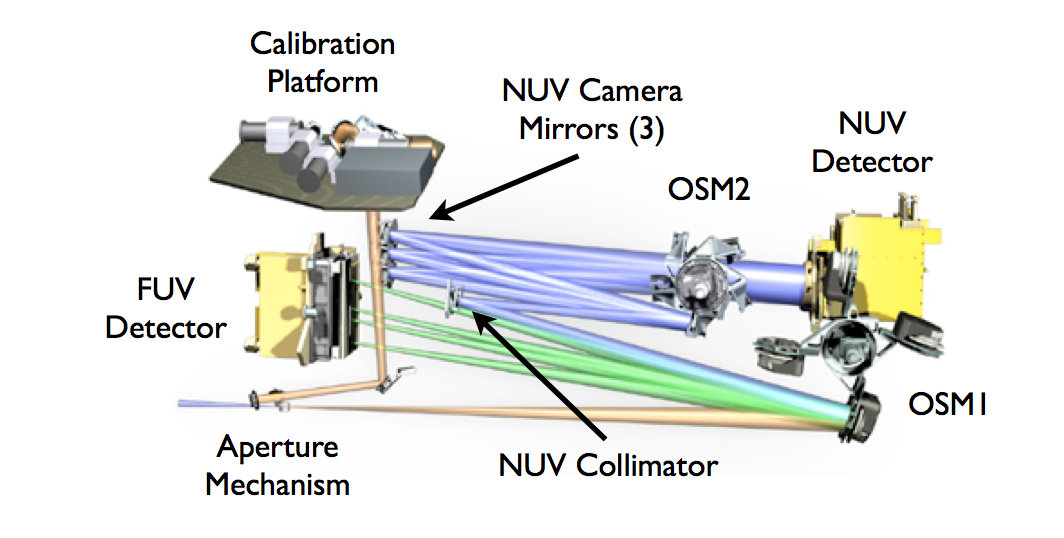
\includegraphics[width=\linewidth]{cos_optical.png}
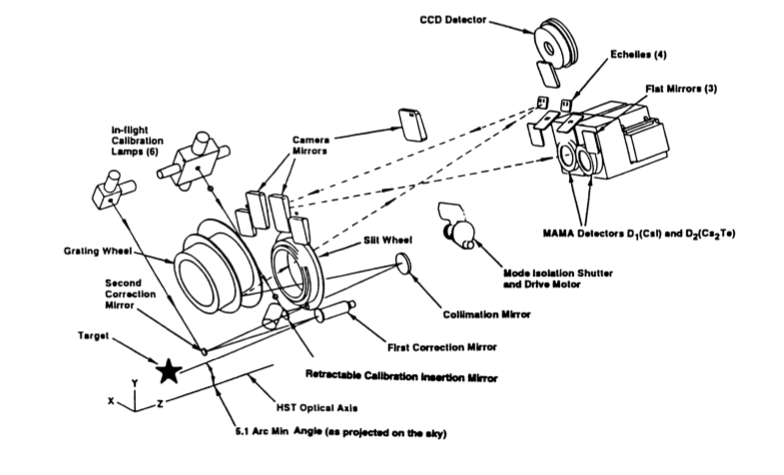
\includegraphics[width=\linewidth]{stis_optical.png}
\caption{Picture are the optical paths and elements of the two spectrographs on HST.  Though built on similar principles, the designs are very different.  \textit{(Top)} COS optical path.
\textit{(Bottom)} STIS optical path.}
\label{fig:x1d_2}
\end{minipage}
\end{figure}

%\begin{figure}[htbp!]
%\begin{center}
%\begin{minipage}[b]{.9\linewidth}
%\begin{center}
%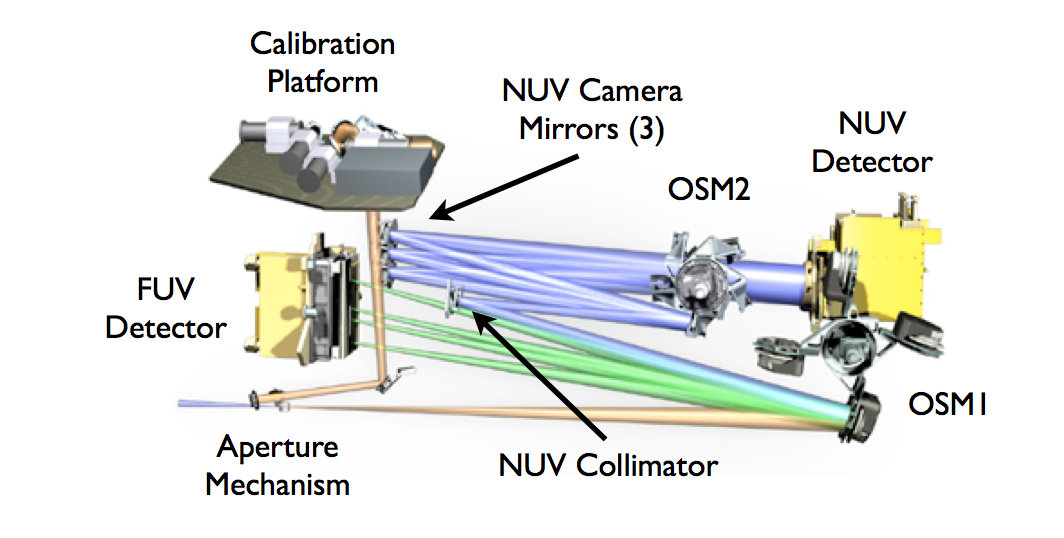
\includegraphics[width=\linewidth]{cos_optical.png}
%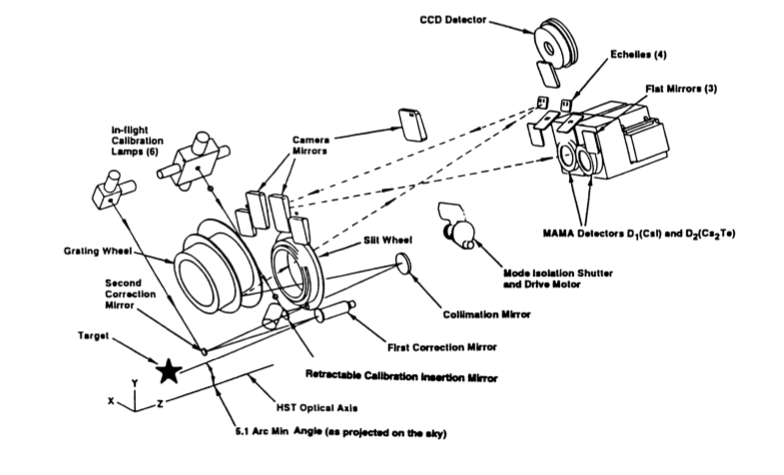
\includegraphics[width=\linewidth]{stis_optical.png}
%\caption{Picture are the optical paths and elements of the two spectrographs on HST.  Though built on similar principles, the designs are very different.  \textit{(Top)} COS optical path.
%\textit{(Bottom)} STIS optical path.}
%\label{fig:x1d_2}
%\end{center}
%\end{minipage}
%\end{center}
%\end{figure}

\section{Uses of Spectroscopy}
Spectroscopy is a very powerful tool used to probe the inner workings of distant objects.  It allows astronomers to measure chemical composition, redshifts, relative velocities, absorption systems, to name a few.

\section{Space-Based Spectroscopy}
\subsection{So many more wavelengths!}
Astronomy from the ground is inhibited by the Earth's atmosphere.   The elements that make up the atmosphere are only transparent to certain wavelength ranges, and so to observe any of the other ranges one must observe from space. See ~\ref{fig:atmo_trans}.

\begin{center}
\begin{figure}[htbp]
\begin{center}
% scale and angle values to be adjusted
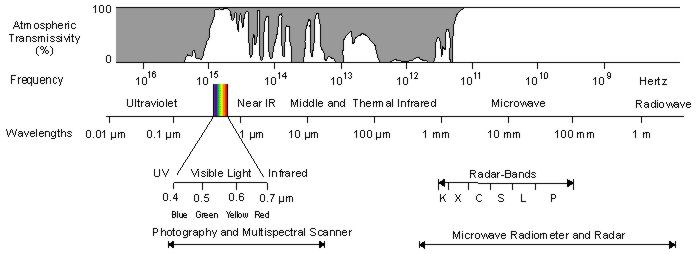
\includegraphics[scale=0.9, angle=0.0]{atmo_trans.jpg}
\caption{Atmospheric transmission with wavelength.  The low transmission at at many wavelengths, particularly UV and shorter, necessitates space based observations.}\label{fig:atmo_trans}
\end{center}
\end{figure}
\end{center}

\subsection{Airglow Lines}
The orbit of HST is close enough to earth to still encounter significant atmospheric effects.  One of the largest of these effects is the presence of emission lines caused by Earth's atmosphere.  The figures below show two of the more prominent lines, Lyman Alpha and Oxygen I.  Both of these features show variability on long and short timescales, with the former changing as HST passes through orbital day and night, and the latter changing as the solar cycle and the earth environment makes large scale changes to atmospheric size, density, etc.  

STIS has the ability to use small slits, and thus to remove much of the contamination from the airglow lines.  COS, however, has a fixed, large, aperture that cannot be used to filter out airglow.  Some filtering can still be done for COS data, but only by removing the part of the exposure that was taken during times of particularly strong airglow emission, such as orbital day. Strong airglow lines have led to the degradation of the COS FUV detector- to combat the damage done, the FUV spectra are periodically shifted up and down in XD (cross-dispersion) to expose on pristine portions of the detector.

\begin{figure}
\begin{minipage}[b]{0.5\linewidth}
\centering
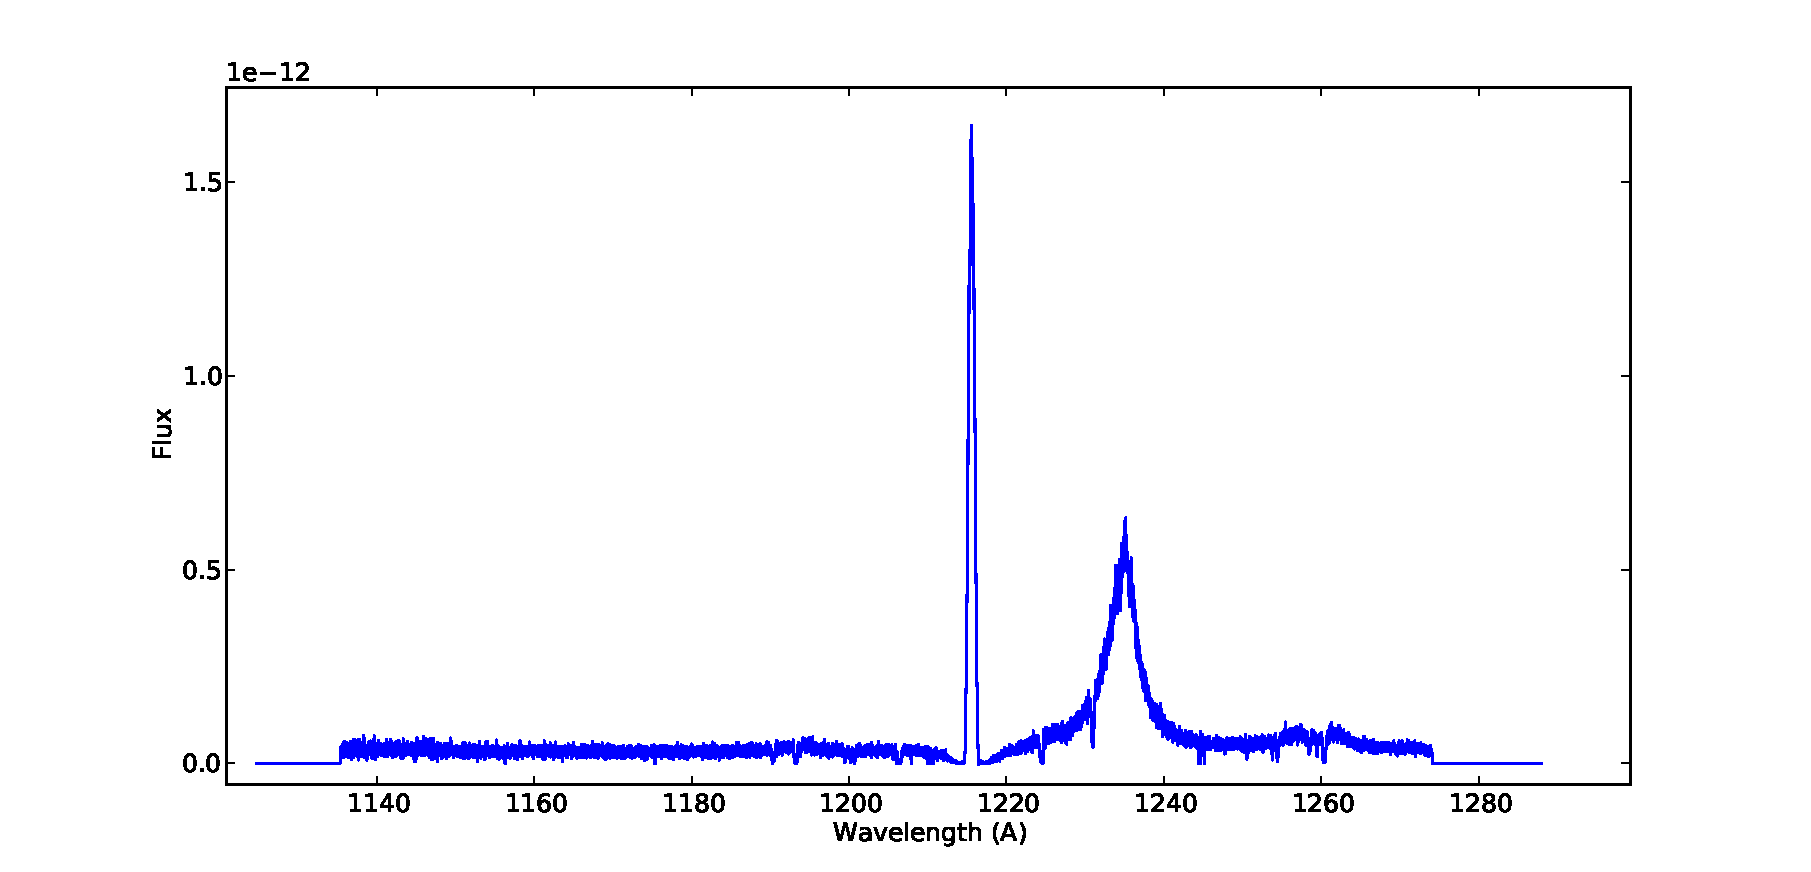
\includegraphics[width=\textwidth]{lya.pdf}
\caption{Geocoronal Lyman Alpha airglow is shown at 1216 \AA.}
\label{fig:geo1}
\end{minipage}
\hspace{0.5cm}
\begin{minipage}[b]{0.5\linewidth}
\centering
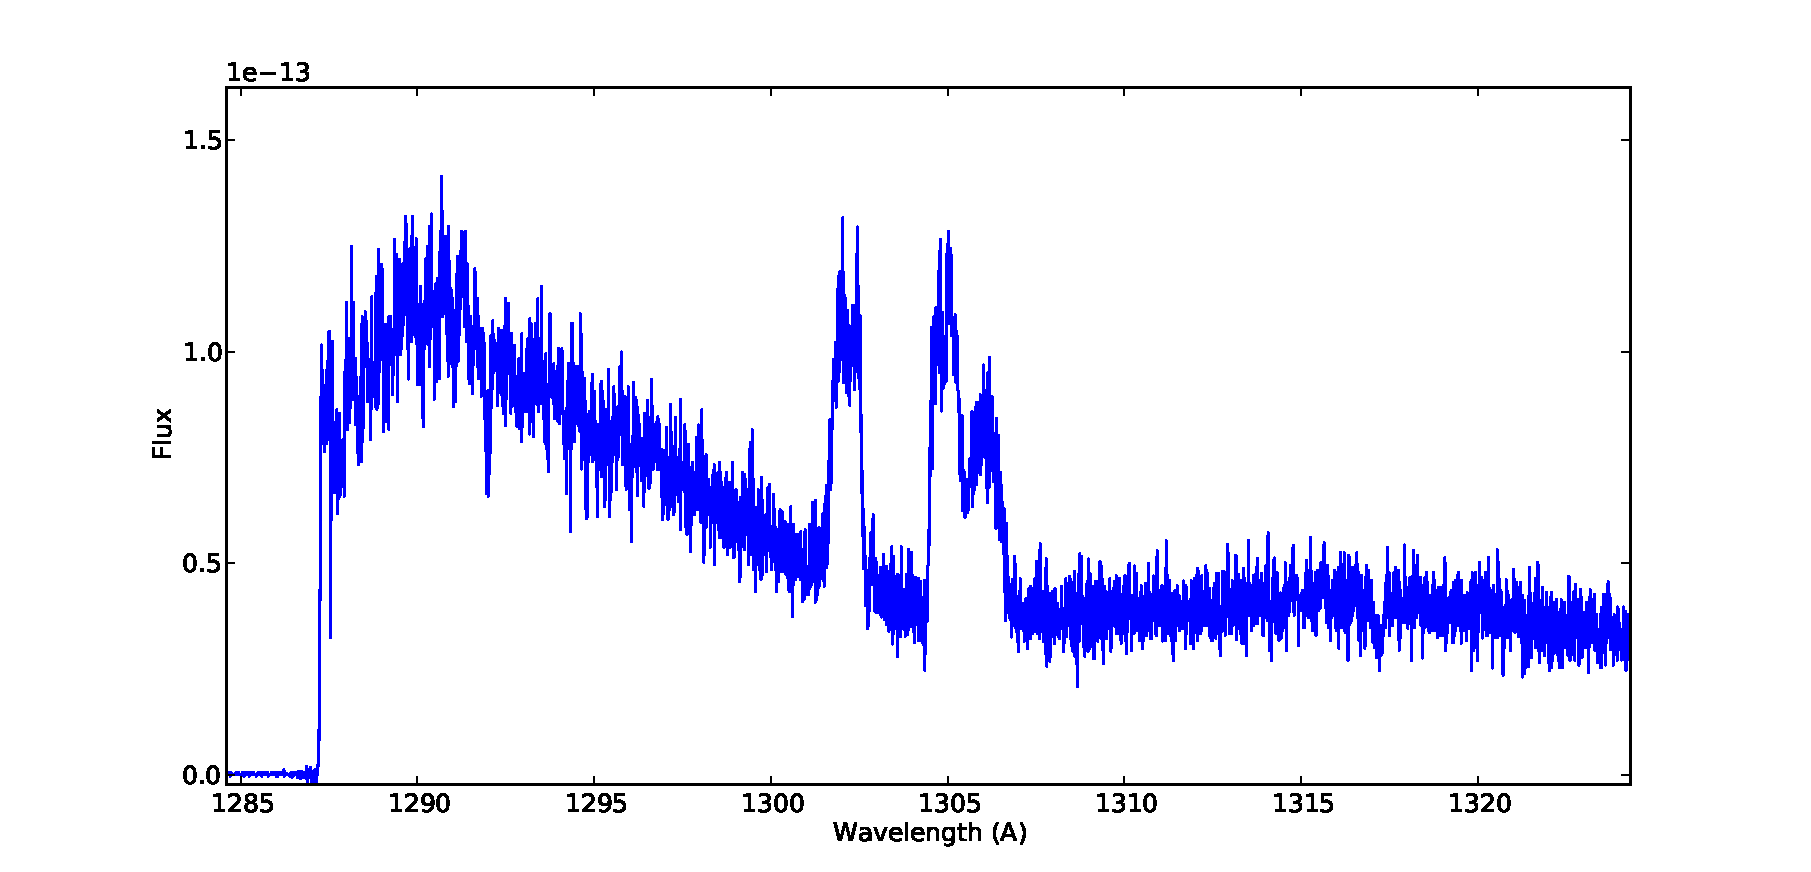
\includegraphics[width=\textwidth]{OIII.pdf}
\caption{Geocoronal Oxygen I airglow between 1300 and 1310 \AA.}
\label{fig:geo2}
\end{minipage}
\end{figure}


\subsection{UV Instrumentation}
Ultraviolet astronomy often requires different detectors than the typical Charged Couple Devices (CCDs).  HST employs two different kinds of UV detectors; Multi-Anode Microchannel Arrays (MAMAs), and an open face Microchannel Plate (MCP) with a Cross Delay Line Anode (XDL).  The MAMA detectors are employed in the FUV and NUV channels of STIS and the NUV channel of COS, \textcolor{red}{while the XDL is only used in the COS FUV channel.} 
%with the XDL only being used in the COS FUV channel.  

These detectors act very differently when compared to CCDs.  The most glaring difference is that these detectors are photon-counting devices.  This means that each incoming photon is uniquely observed by the instrument electronics.  This allows for some great flexibility, and great complexity, in processing of the data.  Data taken in TIME-TAG mode (default on COS, optional on some STIS modes), records the location and time of each photon event.  This means that data can later be screened not just in x,y location, but in time as well.  

UV detectors also experience an incredibly low background rate.  The FUV detector on COS, for example, has a mean dark count rate of $\sim 3.0x10^{-6} cnts/sec/pixel$.   To put this in perspective, in even very long exposures most pixels in the COS FUV detector do not have a single dark count.  

For a far more complete introduction to COS and STIS, along with any other HST instrument, please see that instrument's Instrument Handbook.

\subsection{Differences between COS and STIS}
While both of HST's spectrographs, COS and STIS, overlap in spectral range, there are still many unique advantages to each instrument that will dictate which is the best choice to achieve a program's goals. The FUV throughput, spectral resolution, and wavelength coverage of most COS modes is much higher than that of STIS. In addition, new "blue mode" COS configurations allow observations from the hydrogen Lyman limit (912 \AA) to Ly$\alpha$ (1216 \AA), far surpassing the wavelength range of STIS. The NUV capabilities of both instruments are comparable with the exception that it is easier to obtain broader NUV wavelength coverage with STIS. Generally speaking, STIS is better suited for observing extended sources than COS. Conversely, the COS instrument is optimized to observe point-source objects. The high-dispersion echelle modes of STIS offer resolving powers of up to $R \sim 200,000$. The significantly lower dark rates of COS make it a better choice when observing faint sources. 

Both detectors, however, share a number of features. Both instruments can observe using TIME-TAG mode, recording the time of each photon's arrival. Both COS and STIS MAMA detectors have brightness limits that ensure the safety of the instruments.
\chapter{NumPy and Data Arrays}
\label{ch:numpy}

\section{The Uses of NumPy }
NumPy is a Python module which adds support for large,
multi-dimensional arrays and matrices, along with a large library of
high-level mathematical functions to operate on these arrays. NumPy
addresses the problems of speed in interpreted languages by providing
multi-dimensional arrays and lots of functions and operators that
operate on arrays. Any algorithm that can be expressed primarily as
operations on arrays and matrices can run almost as fast as the
equivalent C code.

\subsection{NumPy's array vs. Python's built-in list}
NumPy introduces new data types, but the most popular, versatile, and
useful one is the array.  This is similar to arrays in IDL.  There
are several reasons why you would want to use a NumPy array over
Python's built-in list.
\begin{itemize}
\item NumPy, PyLab, SciPy, PyFITS and other modules' functions often
  work with NumPy arrays.
\item Every item in a NumPy array is of the same data type.  This
  means there is less information to keep track of which makes array
  computations faster.
\item NumPy arrays act as vectors and therefore we can do things such
  as element-wise addition and multiplication.
\end{itemize}

To convert a list to an array, use {\sf \small numpy.array()}.

%%%%%%%%%%%%%%%%%%%%%%%%%%%%%%%%%%%%%%%%  numpy.array
\subsection{ {\sf numpy.array() } function}
  {\color{blue} {\sf\small USE}} \\
  The {\sf\small numpy.array()} function converts a list to a NumPy
  array.  

{\color{blue} {\sf\small EXAMPLES}} \\
\begin{alltt}
\pytab import numpy as np
\pytab a = [1,2,3,4]      #a python built in list 
\pytab b = np.array(a)     #converted to a NumPy array 
\pytab print a 
\pytab print b 
\pytab indx = [1,2] 
\pytab print b[indx]  
\pytab print b[1:3]       #prints elements 1 to 2, NOT 1 to 3.  
\pytab print b[:3], b[3:] #prints up to the 3rd element, \textbackslash
\ldots    and then everything after the 3rd element.
\pytab print b[-1],b[-2] 
\pytab print b[::-1]      #reverses the array.  
\pytab c = np.array([[1,2,3,4,5],[6,7,8,9,10]]) 
\pytab print c 
\pytab print c[1,3]       #indices for a multi-dimensional array 
\pytab print c[1][3]      #this is slower than the previous as it \textbackslash
\ldots    creates a new array, $c[1]$, and then subscripts that array.
\pytab print c[1,:]  #print the first element in the first \textbackslash
\ldots    dimension, but all in the second dimension
\pytab print c[:,1] 
\end{alltt}
Notice when we print lists and arrays that the elements in lists are
separated by commas while the elements in arrays are only separated by
spaces.

{\color{blue} {\sf\small EXERCISES}} \\
{\it Exercise \arabic{exercise} \stepcounter{exercise}:  \\
  Create a list $a$ and a NumPy array $b$.  Multiply each by 2 and
  explain what happens.  Now add 2 to each array.  Again, explain the
  result.  } \\
{\it Exercise \arabic{exercise} \stepcounter{exercise}:  \\
  Create a third list $c$.  Add $c$ to both $a$ and
  $b$.  Explain the result.}

\section{What a NumPy array really is and a word of caution}

A final note about NumPy arrays is that an array is actually
an object which points to a block of memory.  For example, in the
above exercise we created an array $b$.  Try the following:

\texttt{\pytab d = b}

Now we just created a second array, $d$.  Instead of using up twice
the memory space, $d$ is just a pointer to the memory $b$ also points
to (remember, we copied an array, and an array is a pointer).  Again,
try the following:
\begin{alltt}
\pytab d[2] = 999 
\pytab print d 
\pytab print b 
\end{alltt}
Notice what happened to $b$.  While it saves on memory space,
programmers have to be careful.  If you know you will want to change
one array and not the other, the correct function to use is {\sf
  numpy.copy()}.

%%%%%%%%%%%%%%%%%%%%%%%%%%%%%%%%%%%%%%%%  numpy.copy
\subsection{ {\sf numpy.copy() } function}
\label{s:copy}
{\color{blue} {\sf\small USE}} \\
The {\sf\small numpy.copy()} function copies the contents of the
memory space the array points to. 

{\color{blue} {\sf\small EXAMPLES}} \\
Try the code below and notice the difference in the results from a
simple $d = b$ assignment.
\begin{alltt}
\pytab import numpy as np
\pytab a = np.array([1,2,3,4,5,6,7]) 
\pytab b = a.copy()  
\pytab b[2] = 999  
\pytab print b  
\pytab print a
\pytab a.size
\pytab a.shape
\end{alltt}

\section{Other Common NumPy Functions}
%%%%%%%%%%%%%%%%%%%%%%%%%%%%%%%%%%%%%%%%  numpy.arange
\subsection{ {\sf numpy.arange() } function}
{\color{blue} {\sf\small USE}} \\
The {\sf\small numpy.arange()} function creates an integer array
from zero to the `stop' parameter given, with a step size of one.
The `start' and `step' can also be specified.  By setting the parameter
`dtype' we can change the data type of the array (i.e. to float).

{\color{blue} {\sf\small EXAMPLES}} 
\begin{alltt}
\pytab import numpy as np 
\pytab np.arange(10) 
\pytab 1 + np.arange(10, dtype=float) * 4 
\pytab np.arange(1,40,4,dtype=float)
\end{alltt}
{\color{blue} {\sf\small SEE ALSO}} \\
A similar function for lists is {\sf\small range()}.

{\color{blue} {\sf\small EXERCISES}} \\
{\it Exercise \arabic{exercise} \stepcounter{exercise}:  \\
Create the  sequence 0.1, 0.2,0.3, ... 1.4  using {\sf\small
  numpy.arange()}.  Hint: As noted in the NumPy documentation for
numpy.arange(), it is best to use integer step sizes.} \\
{\it Exercise \arabic{exercise} \stepcounter{exercise}:  \\
Create the  sequence -3.2, -3.0, -2.8, ... -1.0  using {\sf\small
  numpy.arange()}.  See above hint.}

%%%%%%%%%%%%%%%%%%%%%%%%%%%%%%%%%%%%%%%%  numpy.empty
\subsection{ {\sf numpy.empty() } function}
{\color{blue} {\sf\small USE}} \\
The {\sf\small numpy.empty()} function creates a float array of the
specified dimensions. Each element of the array is whatever was left
in that memory space, therefore it is fast but useful only if you know
you will assign each element a meaningful value.
  
{\color{blue} {\sf\small EXAMPLES}} 
\begin{alltt}
\pytab import numpy as np 
\pytab np.empty(10)   #pass an argument, which is the dimensions
\pytab np.empty((3,4)) #here it is 2D, so the dimensions \textbackslash
\ldots    we pass is a tuple
\end{alltt}

{\color{blue} {\sf\small SEE ALSO}} \\
Other useful similar functions are {\sf\small numpy.zeros(), numpy.ones()}.

%%%%%%%%%%%%%%%%%%%%%%%%%%%%%%%%%%%%%%%%  numpy.where
\subsection{ {\sf numpy.where() } function}
{\color{blue} {\sf\small USE}} \\
The {\sf\small numpy.where()} function returns an array (or a tuple of
arrays) of the indices where the condition is $True$.  Otherwise, if you
specify substitute values, it will return an array of the same shape as
the original with the first value substituted where the condition is
$True$, and the second value substituted where the condition is $False$.
  
{\color{blue} {\sf\small EXAMPLES}} 
\begin{alltt}
\pytab import numpy as np
\pytab a = np.arange(11, dtype=float) + 1
\pytab b = np.where(a >= 8.) 
\pytab print b 
\pytab a[b] 
\pytab a = np.array([1,2,3,1,2,1,1,1,1,4]) 
\pytab b = np.where(a == 1, 1,0) 
\pytab print b 
\end{alltt}
If we do not need the indices from {\sf\small numpy.where()} then we
can just use creative indexing for the same effect.
\begin{alltt}
\pytab a > 5
\pytab a[a>5]
\end{alltt}

{\color{blue} {\sf\small SEE ALSO}} \\
Other useful similar functions are {\sf\small numpy.any(),
  numpy.all(), numpy.nonzero(), numpy.choose()}.
 
{\color{blue} {\sf\small EXERCISES}} \\
{\it Exercise \arabic{exercise} \stepcounter{exercise}:  \\
Create a random real 10-element array with numbers between 0 and 1.
Select those with counts lower than 0.5.}


\chapter{Handeling FITS files and ASCII data tables using Astropy}
\label{ch:fits}
Astropy is a python library for astronomy developed by professional astronomers
and software developers from around the world, some of which work here at STScI
in the Science Software Branch.  It is under continuous development and is quickly
becoming a powerful library, especially for handeling FITS files and ASCII tables.
Visit the website listed in Chapter~\ref{ch:links} for more information and useful
documentation.

The astropy.io.fits module provides an interface to FITS formatted files under the 
Python scripting language.  astropy.io.fits data structures are a subclass of NumPy 
arrays, which means that they can use NumPy arrays' methods and attributes.  The
astropy.io.ascii module provides flexible and easy-to-use methods for reading and 
writing ASCII data tables.  In the following sections, we will explore these two modules.
 
\section{Opening, Reading, and Closing a FITS File}
As an example, we will use data from the \emph{NICMOS} instrument located here:  \\
/grp/jwst/wit/miri/randers/PythonTraining/n9vf01hfq\_ima.fits \\ 
Please copy this file to your working directory. 

Below we show an example of opening a FITS file, getting
the data and the header, closing the file, printing out the shape of
the data using {\sf \small numpy.shape}, printing out header values,
and finally making changes to the data.

\begin{alltt}
\pytab from astropy.io import fits
\pytab infile = 'n9vf01hfq_ima.fits'
\pytab fits.info(infile)
\pytab data = fits.getdata(infile, 1) 
\pytab hdr = fits.getheader(infile, 0) 
\pytab data.shape
\pytab print hdr 
\pytab hdr['DARKCORR'] 
\pytab hdr['DARKCORR'] = 'PERFORM'
\pytab hdr['DARKCORR']
\pytab print data[-2:]  #print the last two lines.
\pytab data[-1:][0][0] = 0
\pytab print data[-1]
\end{alltt}

Notice that $hdr$ behaves like a dictionary.  We did some
bad things to this file, but let's save it anyway to a new file.

\begin{alltt}
\pytab outfile = 'mybad.fits'
\pytab fits.writeto(outfile, data, hdr)
\pytab print 'Saved FITS file to: {}'.format(outfile)
\end{alltt}

Alternatively, if we want to modify the original file directly,
we can do the following:

\texttt{\pytab fits.update(infile, data, 1)}

\section{{\sf fits.getval()} and {\sf fits.setval()} functions}

If you are familiar with IRAF, you are probably familiar with IRAF's
{\sf\small hedit} function, which allows you to add, delete, and
modify keywords in a FITS header.  

First, lets take a look of our example file's header using {\sf\small
  imheader} in PyRAF.  In PyRAF navigate to the folder where your
n9vf01hfq\_ima.fits file is located, and try the following:

\begin{alltt}
--> imheader n9vf01hfq_ima.fits[0] l+ | page 
\end{alltt}

We see that there is a 'NSLEWCON' keyword, and it is set to 'Clear.'
Using {\sf\small hedit} we can change the 'NSLEWCON' keyword from
'Clear' to 'Set' as shown here:

\begin{alltt}
--> hedit n9vf01hfq_ima.fits[0] NSLEWCON 'Set'  \textbackslash
\ldots     verify=no update=yes
\end{alltt}

In the above example we made sure the 'update' parameter was set to
'yes.'  We can check that our edit was successful by using  {\sf\small
  imheader} again:

\begin{alltt}
--> imheader n9vf01hfq_ima.fits[0] l+ | page 
\end{alltt}

Without using IRAF, there is a simple way to do this in astropy using
{\sf\small fits.getval()} and {\sf\small fits.setval()}, shown in
the example below.

\begin{alltt}
\pytab from astropy.io import fits
\pytab infile = 'n9vf01hfq_ima.fits' 
\pytab key = 'NSLEWCON'
\pytab fits.getval(infile, key, 0)
\pytab fits.setval(infile, key, value='Clear', ext=0)
\pytab fits.getval(infile, key, 0)
\end{alltt}

Now our FITS file is back to its 'initial' state.  No harm done.


\section{Reading and Writing ASCII Data Files}

The astropy.io.ascii module provides two robust methods, ascii.read() and
ascii.write(), for reading and writing multi-column delimited data tables,
respectively.
\chapter{Plotting with Pyplot}
\label{ch:pyplot}

\section{matplotlib.pyplot}
Matplotlib and its PyPlot environment is a versatile Python plotting
library which produces publication quality figures in a variety of
hard-copy formats such as EPS, PDF, and PNG.  With PyPlot you can
generate scatter and line plots, histograms, power spectra, bar
charts, error-charts, pie charts, and many more with just a few lines
of code. For the power user, you have full control of line styles,
font properties, axes properties, and so on. For useful examples of 
astronomy plots that can be generated with PyPlot, see Leonardo 
Ubeda's astroplotlib library at \href{http://astroplotlib.stsci.edu/}
{http://astroplotlib.stsci.edu/}


\section{Create a Simple Scatter Plot}

We'll start by making a simple scatter plot, demonstrating some of 
the PyPlot options, and saving our plot in a PDF format. 

First, we need to read in some data, as we learned in Chapter~[[...]].

\begin{alltt}
\pytab from astropy.io import ascii
\pytab data_A = ascii.read('flux_vs_time_A.dat', names=['Time',  \textbackslash 
\ldots 'Flux_pcnt_diff', 'Flux_err', 'Flux_linear_fit'])
\pytab data_C = ascii.read('flux_vs_time_C.dat', names=['Time',  \textbackslash 
\ldots 'Flux_pcnt_diff', 'Flux_err', 'Flux_linear_fit'])
\end{alltt}

The time is in Modified Julian Date (MJD) and the remaining 
columns are flux percent differences and are dimensionless. 
(The fluxes are of a standard white dwarf for a WFC3 monitoring 
program. The two datasets are from different amplifiers
on the WFC3 two-chip mosaic.)

Now we will import PyPlot and make our first plot, 
using a \textit{figure} object...

\begin{alltt}
\pytab import matplotlib.pyplot as pyplot
\pytab figure, ax = pyplot.subplots()
\end{alltt}

Now we can begin to plot into the \textit{figure} object, via the \textit{ax} 
axis created in the previous step. Each subsequent call to the inherited 
\textit{ax.plot} method will update the overall plot. The next two calls
plot the two sets of flux differences as scatter plots in blue and red,
respectively.

\begin{alltt}
\pytab ax.scatter(data_A['Time'], data_A['Flux_pcnt_diff'], c='blue')
\pytab ax.scatter(data_C['Time'], data_C['Flux_pcnt_diff'], c='red')
\pytab figure.show()
\end{alltt}

The \textit{figure.show()} command displays our changes onto the \textit{figure}
object.

We should add axis labels...

\begin{alltt}
\pytab ax.set_xlabel('Time [MJD]', fontsize=20)
\pytab ax.set_ylabel('Flux Diff [%]',  fontsize=20)
\pytab figure.show()
\end{alltt}

Finally let's save the figure. We can save as a PDF, PNG, TIFF, and
other file types; we need only to type the appropriate extension.

\begin{alltt}
\pytab figure.savefig('flux_vs_time_1.pdf')
\end{alltt}


%%%%%%%%%%%%%%%%
\begin{figure}[tbp]
  \centering
    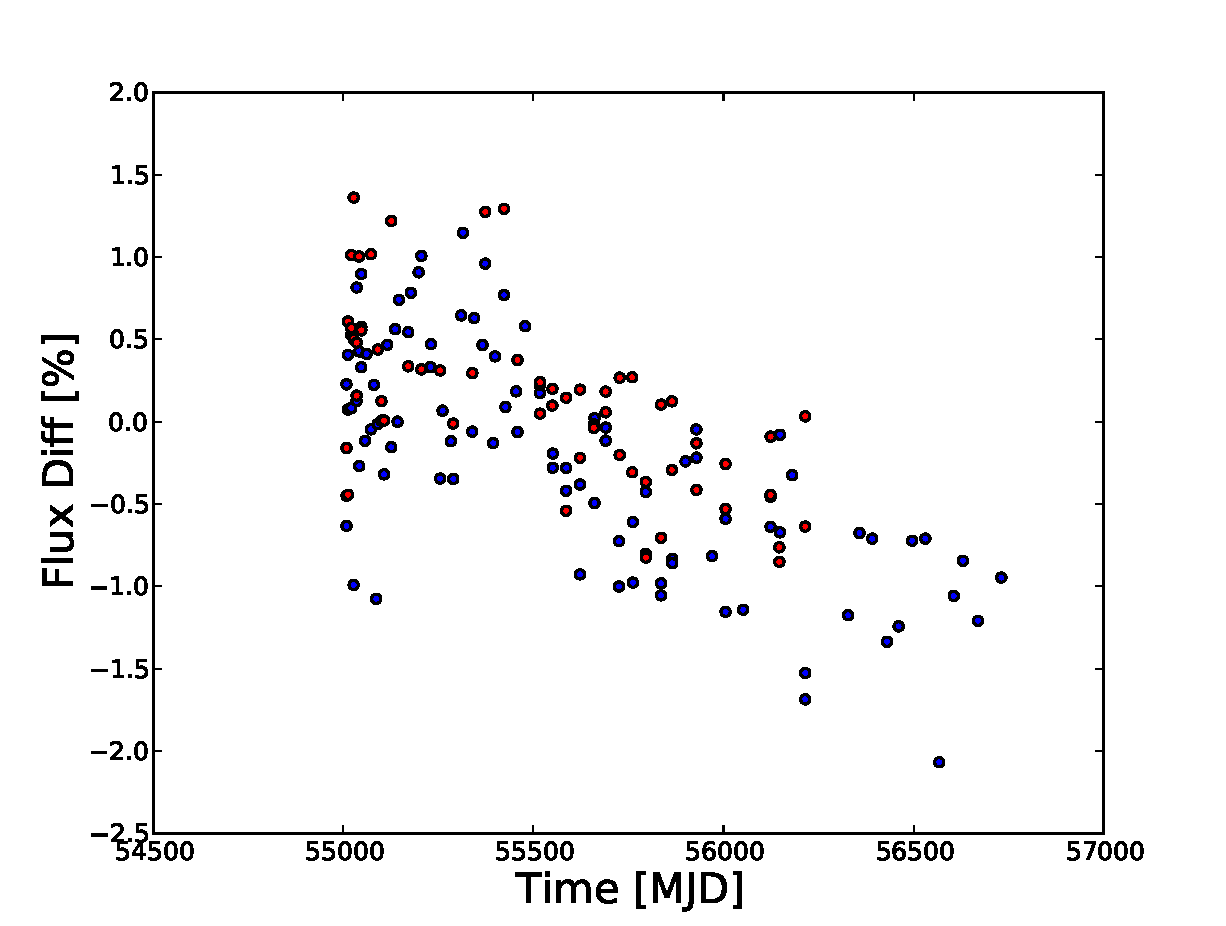
\includegraphics[scale=0.55]{flux_vs_time_1.pdf}
    \caption{Our first plot.}
  \label{fig:splot}
\end{figure}
%%%%%%%%%%%%%%%%

\section{Markers, Lines, and Legends}  %Plot customizations

We have a plot! But we are not yet finished.
PyPlot has many, many options available for you to customize
your plot. We'll demonstrate just a few for markers, lines, and legends. 

We can play with the marker type (\textit{marker}), size (\textit{s}), and 
transparency (\textit{alpha}) of our of scatter plots' points. We first
need to clear the figure with the \textit{ax.clear()} command.

\begin{alltt}
\pytab ax.clear()
\pytab ax.scatter(data_A['Time'], data_A['Flux_pcnt_diff'], \textbackslash 
\ldots   c='blue', marker='x', s=30, alpha=0.75)
\pytab ax.scatter(data_C['Time'], data_C['Flux_pcnt_diff'], \textbackslash 
\ldots   c='red', marker='d', s=30, alpha=0.75)
\pytab ax.set_xlabel('Time [MJD]', fontsize=20)
\pytab ax.set_ylabel('Flux Diff [%]', fontsize=20)
\pytab figure.show()
\end{alltt}

The plot would be clearer if we added a legend.

\begin{alltt}
\pytab ax.clear()
\pytab ax.scatter(data_A['Time'], data_A['Flux_pcnt_diff'], \textbackslash 
\ldots   c='blue', marker='x', s=25, alpha=0.75, label='Amp A')
\pytab ax.scatter(data_C['Time'], data_C['Flux_pcnt_diff'], \textbackslash 
\ldots   c='red', marker='d', s=25, alpha=0.75, label='Amp C')
\pytab ax.set_xlabel('Time [MJD]', fontsize=20)
\pytab ax.set_ylabel('Flux Diff [%]', fontsize=20)
\pytab ax.legend(loc='best', scatterpoints=1)
\pytab figure.show()
\end{alltt}

The \textit{ax.legend(loc='best')} command will try to find the least busy section 
of your plot and stick the legend there. 

Next let's plot lines with the linear fits from our data:

\begin{alltt}
\pytab ax.plot(data_A['Time'], data_A['Flux_linear_fit'], \textbackslash 
\ldots  c='blue', ls='--', linewidth=2, label='Amp A Fit')
\pytab ax.plot(data_C['Time'], data_C['Flux_linear_fit'], \textbackslash 
\ldots  c='red', ls=':', linewidth=2, label='Amp C Fit')
\pytab ax.legend(loc='best', scatterpoints=1)
\pytab figure.show()
\end{alltt}

Suppose we want to denote the 0.0 flux difference with a dashed line and the
MJD date 56250.0 with a green line:

\begin{alltt}
\pytab ax.axhline(0.0, color='k', ls='--', linewidth=1)  
\pytab ax.axvline(56250.0, color='green', ls='-', linewidth=2) 
\pytab figure.show()
\end{alltt}

%%%%%%%%%%%%%%%%
\begin{figure}[tbp]
  \centering
    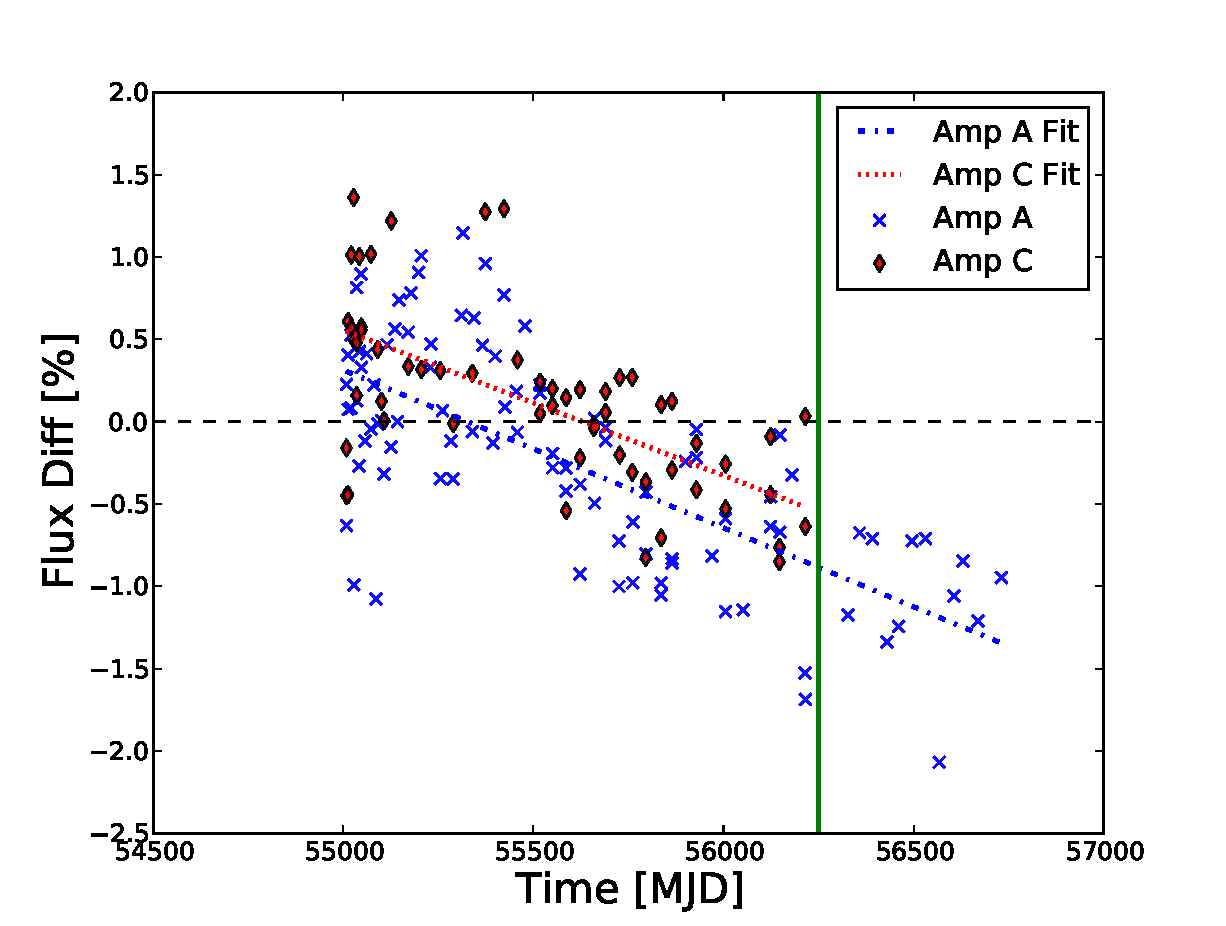
\includegraphics[scale=0.55]{flux_vs_time_2.pdf}
    \caption{Our customized plot.}
  \label{fig:splot}
\end{figure}
%%%%%%%%%%%%%%%%

We now have a personalized plot! (It doesn't have to be pretty.) Let's save it.

\begin{alltt}
\pytab figure.savefig('flux_vs_time_2.pdf')
\end{alltt}

Other options can be found on the Matplotlib PyPlot site listed in Chapter~\ref{ch:links}. 

For different color names, see \href{http://www.w3schools.com/html/html_colornames.asp}
{http://www.w3schools.com/html/html\_colornames.asp}

%http://matplotlib.org/1.2.1/examples/pylab_examples/show_colormaps.html


\section{Error Bars}

We have columns giving our error. We can display them on our plot as
error bars using the \textit{errorbar} function:

\begin{alltt}
\pytab ax.clear()
\pytab ax.scatter(data_A['Time'], data_A['Flux_pcnt_diff'], c='blue')
\pytab ax.errorbar(data_A['Time'], data_A['Flux_pcnt_diff'], \textbackslash 
\ldots yerr=data_A['Flux_err'], c='grey', marker=None, ls='None')
\pytab figure.show()
\end{alltt}


\section{Display Dates on X-axis}

MJD is a convenient format for plotting time. But who 
thinks in MJD? Let's convert it to dates and display them 
on the x-axis. In python this is a little tricky.



\section{Plot Figures Side-by-Side}

%many examples from ...


\section{Fitting Lines}



\section{Display a FITS Image}
%Different examples of drawing over image.


\section{Plot Spectra}








\section{Plot with Pyplot}
From Section~\ref{ss:loadtxt} we learned how to read in data from a
file, particularly Gordon2005\_Fig16.txt.  We will reproduce the slope
plot in Figure~16 of the Gordon 2005 paper.

\begin{alltt}
\pytab import numpy as np 
\pytab infile = 'Gordon2005_Fig16.txt' 
\pytab slope, ran_slope_unc, corr_slope_unc, \textbackslash 
\ldots      both_slope_unc, eqn_slope_unc = np.loadtxt(infile, 
\ldots      usecols=(0, 1, 2, 3, 4), unpack=True) 
\end{alltt}

These arrays have nice descriptive names, but to help make the
plotting process clear, we will assign short names.

\begin{alltt}
\pytab xx = slope  
\pytab yy1 = ran_slope_unc  
\pytab yy2 = corr_slope_unc  
\pytab yy3 = both_slope_unc
\pytab yy4 = eqn_slope_unc 
\end{alltt}

Now we will import Pyplot and make our first plot, using a \textit{figure} 
object...

\begin{alltt}
\pytab import matplotlib.pyplot as plt  
\pytab figure, ax = plt.subplots()
\end{alltt}

Now we can begin to plot into the \textit{figure} object, via the \textit{ax} 
axis created in the previous step. Each subsequent call to the inherited 
\textit{ax.plot} method will update the overall plot... 

\begin{alltt}
\pytab ax.plot(xx, yy1, ls='--', color='b')
\pytab ax.plot(xx, yy2, ls=':', color='r')
\pytab ax.plot(xx, yy3, ls='-', color='g')
\pytab ax.plot(xx, yy4, ls='-.', color='m')
\end{alltt}

Notice that `b' is for blue, `r' is for red, `g' is for green, and `m'
is for magenta.  Furthermore, `-' is for a solid line, `--' is for a
dashed line, `:' is for a dotted line, and `-.' is for a dot-dash
line.  Several other options are available as well and can be found on
the Matplotlib Pyplot site listed in Chapter~\ref{ch:links}. 

The lines are pretty faint, and we also need to add a legend and axis
labels. Let's start by clearing the \textit{axis} object, replotting, and then 
force a refresh on our \textit{figure}:

\begin{alltt}
\pytab ax.clear()
\pytab ax.set_xlabel('Slope [e-/s]')
\pytab ax.set_ylabel('Slope Uncertainty [e-/s]')
\pytab ax.plot(xx, yy1, ls='--', color='b', label='Randon Unc.')
\pytab ax.plot(xx, yy2, ls=':', color='r', label='Correlated Unc.')
\pytab ax.plot(xx, yy3, ls='-', color='g', label='Both')
\pytab ax.plot(xx, yy4, ls='-.', color='m', label='Equation')
\pytab ax.legend(loc='best')
\pytab figure.show()
\end{alltt}

We can save this plot.  The figure will save as a PDF, PNG, TIFF, and
others depending on the name given.

\begin{alltt}
\pytab figure.savefig('fig16.pdf')
\pytab figure.clf()
\end{alltt}

Notice that we cleared the figure with \textit{figure.clr()}. This step is not 
necessary, but is useful to clear a figure object that is no longer needed. 
Open fig16.pdf and take a look.  It looks pretty good, right?

\begin{figure}[tbp]
  \centering
    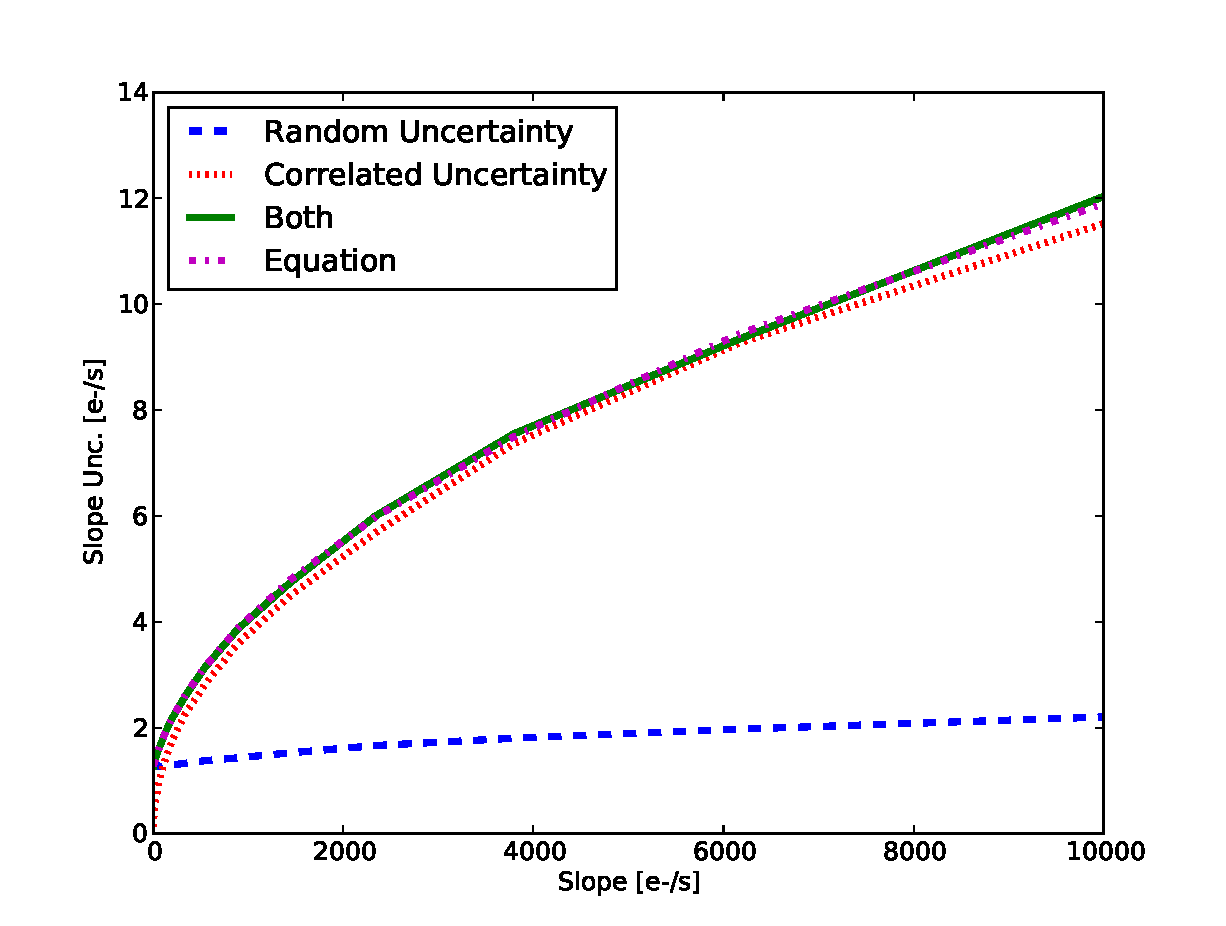
\includegraphics[scale=0.55]{splot.pdf}
    \caption{Our first try at re-creating Figure 16 in Gordon 2005.}
  \label{fig:splot}
\end{figure}

If you look at the paper by
Gordon et al. 2005, though, you will see that the key thing we are missing is
logarithmic axis.  Instead of \textit{matplotlib.pyplot.plot} we will use \textit{matplotlib.pyplot.loglog}:

\begin{alltt}
\pytab ax.clear()      # Clear the axis...
\pytab ax.loglog(xx, yy1, ls='--', lw=3, color='b', label='Random Unc.')
\pytab ax.loglog(xx, yy2, ls=':', lw=3, color='r', label='Correlated Unc.')
\pytab ax.loglog(xx, yy3, ls='-', lw=3, color='g', label='Both')
\pytab ax.loglog(xx, yy4, ls='-.', lw=3, color='m', label='Equation')

\pytab ax.set_xlabel('Slope [e-/s]')
\pytab ax.set_ylabel('Slope Uncertainty [e-/s]')
\pytab ax.legend(loc='best')
\pytab figure.show()
\end{alltt}

Again, open the figure you just made.  How does that look?  

\begin{figure}[tbp]
  \centering
    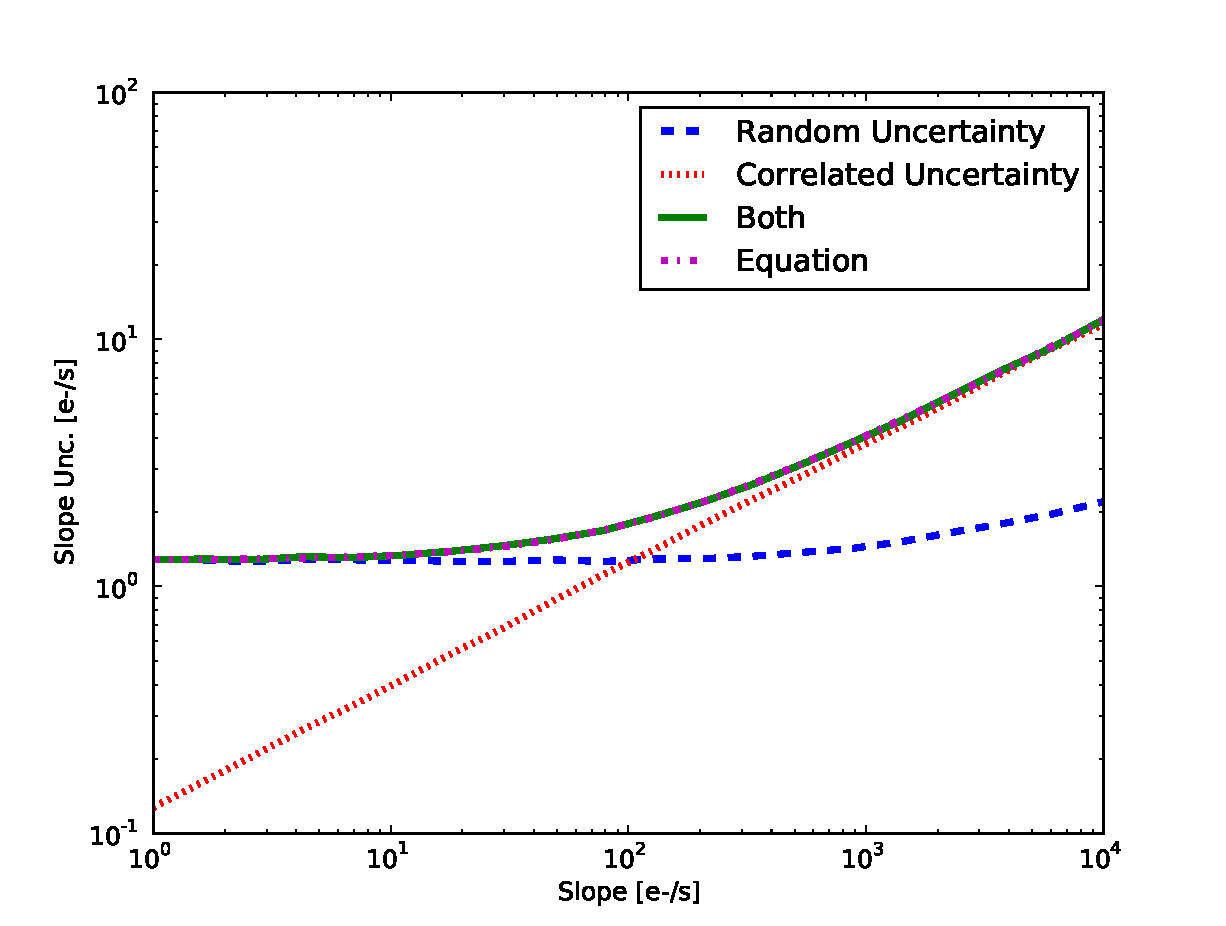
\includegraphics[scale=0.6]{splot_log.pdf}
    \caption{Our version of Figure 16 in Gordon 2005.}
  \label{fig:splot}
\end{figure}

For more
plotting options with Matplotlib and Pyplot, check out the 
\href{http://matplotlib.org/}{matplotlib.org} link listed in
Chapter~\ref{ch:links}.  Notice that there is a link to NumPy on this
page, as well as links to screen-shots, thumbnails, and examples.

Our plot is looking good, however this is getting way too messy.
Isn't there a way we can keep this all nicely in a file, where we can
type it once correctly and never have to type it again?  Sure there
is!  We need to write a script.

\include{notebook}
\chapter{Introduction to PyRAF}
\label{cha:chapter2}


 
\section{What is PyRAF? }
PyRAF is a command language for running IRAF tasks in a Python like environment. It works very similar to IRAF, but has been updated to allow such things as importing Python modules, starting in any directory, GUI parameter editing and help. Most importantly, it can be imported into Python allowing you to run IRAF commands from within a larger script. PyRAF is part of the stsci\_python package and is a product of the Science Software Branch here at STScI. All of the STScI calibration pipelines can be run from PyRAF although they are now written in Python and more recent pipelines (e.g. \emph{Calcos}) can be run as stand-alone programs.

\subsection{IRAF}
IRAF stands for Image Reduction and Analysis Facility and is written and supported by the National Optical Astronomy Observatories (NOAO). It has many tools for both spectroscopic and image analysis. Scripting in IRAF can be done using an IRAF-specific language called ``CL script'', however that will not be covered in this document. Most information covered in this document applies to both IRAF and PyRAF but is generally more user friendly in PyRAF.

\section{Getting Started}

Ensure you have activated the {\tt conda} environment that you set up in the {\bf Computer Setup} section. Create a {\tt login.cl} file to configure IRAF by running {\tt mkiraf} in your home directory. When asked to {\tt Initialize uparm?}, answer {\tt y}. When prompted to {\tt Enter terminal type}, you should supply {\tt xterm}.

If the command {\tt mkiraf} is not available, use {\tt conda install -c http://ssb.stsci.edu/conda-dev/ iraf pyraf}. Packaging for PyRAF and IRAF is currently transitioning to a new system, so check with your trainer if the installation does not work.

\section{The Basics}
\subsection{Navigation}
PyRAF contains many packages which have to be imported. You import a package by typing the name in the command line. For example, to use the {\bf Calstis} function I need to have the {\bf stis} packge loaded which is in the {\bf hst\_calib} package, which is in the {\bf stsdas} package,  I type the following in a PyRAF window:

\begin{minipage}{4in}
\setlength{\oddsidemargin}{0.25 in}
\setlength{\evensidemargin}{0.25 in}
\begin{tabular}{ll}
& {\color{RoyalBlue}--> stsdas}\\
& {\color{RoyalBlue}--> hst\_calib}\\
&{\color{RoyalBlue}--> stis}\\
\end{tabular}
\end{minipage}

To find out the packages available in your current package type \emph{?}. For example:

\begin{minipage}{4in}
\setlength{\oddsidemargin}{0.25 in}
\setlength{\evensidemargin}{0.25 in}
\begin{tabular}{ll}
& {\color{RoyalBlue}--> stsdas}\\
& {\color{RoyalBlue}--> hst\_calib}\\
& {\color{RoyalBlue}--> ?}\\
\end{tabular}
\end{minipage}

This will tell you all of the packages in {\bf hst\_calib}. Functions with an @ symbol are parameter tables, not functions.

\subsection{Help}
You get help information on any package or function by typing {\bf help function}. This not only tells you about a function, it also tells you the packages that you have to call to get to it. For instance, if you want to use the command {\bf splot}:

\begin{minipage}{4in}
\setlength{\oddsidemargin}{0.25 in}
\setlength{\evensidemargin}{0.25 in}
\begin{tabular}{ll}
& {\color{RoyalBlue}--> help splot}
\end{tabular}
\end{minipage}

This will tell you that {\bf splot} is in the {\bf onedspec} in the {\bf noao} package. This can also be entered in GUI form from the epar GUI. 

\subsection{epar}
All functions have input parameters most of which can either be entered in the command line or can be set in the parameter editor using the epar GUI. If you type: \emph{epar function} you will get a table of all of the parameters. There are 5 buttons at the top of the epar editor: Execute, Save, Unlearn, Cancel, and Help. Execute runs the function with the parameters given, Save exits the epar editor and saves the parameters but doesn't execute the function, Unlearn set all of the parameters to their default values, Cancel exits the epar editor without saving, and Help displays the help file for the function. 

\subsection{Using a List as Input}
Many PyRAF functions cannot use wildcards but can take a file which is a list of files. A file which is a list is distinguished from an input file for processing by using an @ sign at the beginning of the file name. For example if you have 3 files, file1.fits, file2.fits, and file3.fits, you can first make a file which is a list of the file names:

\begin{minipage}{4in}
\setlength{\oddsidemargin}{0.25 in}
\setlength{\evensidemargin}{0.25 in}
\begin{tabular}{ll}
& {\color{RoyalBlue}> ls *.fits > filelist.txt } \\
\end{tabular}


Then use this as the input to the {\bf catfits} function: \\
\begin{tabular}{ll}
& {\color{RoyalBlue}--> catfits @filelist.txt } \\
\end{tabular}
\end{minipage}


\subsection{importing function}
Because PyRAF is Python based, you can import any Python module. This is particularly useful when calibrating a group of datasets as many instrument pipelines (Cal*) will not take wild cards as inputs.  If you are mixing PyRAF and Python commands you often have to put an iraf. infront of the commands to let PyRAF know that your are executing a PyRAF command. In the following example I will import the {\bf glob} module from python and use it to select all of the raw files in a directory. I will then calibrate each raw file (note I use iraf.calstis rather than just calstis).

\begin{minipage}{4in}
\setlength{\oddsidemargin}{0.25 in}
\setlength{\evensidemargin}{0.25 in}
\begin{tabular}{ll}
& {\color{RoyalBlue}> pyraf}\\
& {\color{RoyalBlue}--> import glob}\\
& {\color{RoyalBlue}--> flist = glob.glob('*raw.fits')}\\
& {\color{RoyalBlue}--> for ifile in flist:}\\
\end{tabular}
\setlength{\parindent}{0.5 in}
%\setlength{\parskip}{-0.2 in}

{\color{RoyalBlue}iraf.calstis(ifile)}\\
\end{minipage}

\subsection{Exercises}
\begin{enumerate}
\item In PyRAF locate the package {\bf apextract}. What tasks are in this package? What does the {\bf aptrace} task do? Are there any parameter tasks?
\end{enumerate}


\chapter{Python Scripts and Functions}
\label{ch:scripts}

Make a directory where you will keep all of your scripts.  You will
also need to choose a text editor, such as Emacs, TextWrangler, NEdit,
or others.  You will be using this to edit your scripts.
 
\section{MyFirstScript.py}

Create a file called MyFirstScript.py in your script directory, and
open it in your favorite editor.  Comments in scripts are very
important, not just to help you remember what exactly you were
thinking, but to help others as well should they ever use your code.
Therefore, to start off on the right foot, let's create a special header 
called a docstring that looks something like this:

\begin{verbatim}
' ' '
ABOUT:
This is a program that takes this and plots that.

DEPENDS:
Python 2.5.4

AUTHOR:
M.E. MySelf for STScI, 2011

HISTORY:
2011: Trial program.

USE:
python MyFirstScript.py
' ' '
\end{verbatim}

For the header we show three apostrophes to comment out multiple lines
of text.  Next thing we will want to have is all of our imports.

\begin{verbatim}
import numpy as np
import matplotlib.pyplot as plt 
\end{verbatim}

Now we are ready!  Look back through your shell and create your script
from Chapter~\ref{ch:pylab}.  So far you should have something similar
to the following:

\begin{verbatim}
infile = 'Gordon2005_Fig16.txt'
outfile = 'fig16_log.pdf' 

slope, ran_slope_unc, corr_slope_unc, both_slope_unc,  \
    eqn_slope_unc = np.loadtxt(infile, 
    usecols=(0, 1, 2, 3, 4), unpack=True) 
plt.loglog(slope, ran_slope_unc, 'b--',  
    slope, corr_slope_unc,'r:' , slope, both_slope_unc, 'g-',  
    slope, eqn_slope_unc, 'm-.', linewidth=3) 
plt.legend(('Random Uncertainty','Correlated Uncertainty',  
    'Both','Equation'),'best')
plt.ylabel('Slope Unc. [e-/s]') 
plt.xlabel('Slope [e-/s]') 
plt.savefig(outfile) 
plt.clf()
\end{verbatim}

Notice that we listed any variables (or things we might want to change
later) at the top of the program, such as $outfile$ and $infile$.
Also, since we do not have to type the variables over and over, I
decided to use the more descriptive names.  This will also help if I
do not work on this script for awhile and then later come back to it.
Now our program is ready to execute.

\subsection{Executing Python Scripts}

There are a few ways to run a Python program.  One is to type from your terminal:

\texttt{\termtab python MyFirstScript.py}

Or, if you are already inside the Python interactive environment, just
type:

\texttt{\pytab import MyFirstScript}

For the last example, if you want to re-run the script, type:

\texttt{\pytab reload(MyFirstScript)}

Another way is to make the program executable and then type:

\texttt{\termtab MyFirstScript.py}

This is nice.  You do not have to type `python', you can run it from
anywhere, and you do not have to be in the Python interactive
environment.  However, we must first do two things.
\begin{enumerate}
\item To tell your computer which shell or interpreter should be used
  for executing this file, at the very top of your file add:

  \texttt{\#! /usr/bin/env python}

\item You will need to make your script executable.  In the terminal,
  type:

  \texttt{\termtab chmod a+x MyFirstScript.py}  
\end{enumerate}

To be able to call your script from anywhere on your computer, add
your script directory to your executable path by opening your
.mysetenv file and adding the line (with the correct path substituted
in):

\texttt{setenv PATH .:/my/script/directory:\{\$PATH\}}

Next, in your terminal execute the command:

\texttt{\termtab source .mysetenv}

{\color{blue} {\sf\small EXERCISES}} \\
{\it Exercise \arabic{exercise} \stepcounter{exercise}:  \\
  Write your script MyFirstScript.py and execute it.
}

\section{Adding Functions}
\label{s:fun}
MyFirstScript.py is short and easy to read.  However, we can imagine a
case where we have such a large program and many repeated tasks that
it will become difficult.  For example, if we want to create the
y-intercept uncertainty plot as well as the slope uncertainty plot we
can either repeat several lines of our program (and if we change one
copy remember to change the other), or we can create a plotting
function and just call that function twice.  The general format of
declaring a function and then using it is shown below.

\begin{verbatim}
#! /usr/bin/env python

# Header

def mkplot(data): 
    # Make plot here
    return

if __name__=='__main__':
    data = SomeFunctionThatGetsData()
    mkplot(data)
    print 'Now I have a beautiful plot!'
\end{verbatim}

Notice the line \texttt{if \_\_name\_\_=='\_\_main\_\_':}.  It is often useful
to start the main program with this statement.  In this way you can
make the file usable as a script as well as an import-able module,
because the code that parses the command line only runs if the module
is executed as the `main' file, i.e. `MyFirstScript.py'.  In this way,
from another program (or a Python prompt) we could call

\texttt{from MyFirstScript import mkplot}.   

Let's modify our program to look like this:

\begin{verbatim}
#! /usr/bin/env python

#Header

__author__ = 'M.E. MySelf'
__version__ = 0.2

import numpy as np
import matplotlib.pyplot as plt

def mkplot(outfile,xx,yy1,yy2,yy3,yy4,ylab='Slope Unc. [e-/s]'):
    plt.loglog(xx, yy1, 'b--', xx, yy2, 'r:' , xx, yy3, 'g-', xx,  
        yy4, 'm-.', linewidth=3) 
    plt.legend(('Random Uncertainty','Correlated Uncertainty',  
        'Both','Equation'),'best')
    plt.ylabel(ylab) 
    plt.xlabel('Slope [e-/s]') 
    plt.savefig(outfile) 
    plt.clf()
    print 'Saved file to: ',outfile 
    return  
    
if __name__=='__main__': 
    infile = 'Gordon2005_Fig16.txt' 
    slope_outfile = 'fig16_slope.pdf'  
    yint_outfile = 'fig16_yint.pdf'  
    
    slope, ran_slope_unc, corr_slope_unc, both_slope_unc,  \
        eqn_slope_unc, ran_yint_unc, corr_yint_unc,  \
        both_yint_unc, eqn_yint_unc = np.loadtxt(infile, 
        unpack=True) 
    mkplot(slope_outfile, slope, ran_slope_unc, corr_slope_unc,  
        both_slope_unc, eqn_slope_unc) 
    mkplot(yint_outfile, slope, ran_yint_unc, corr_yint_unc,  
        both_yint_unc, eqn_yint_unc,
        ylab='Y-Intercept Unc. [e-]')
\end{verbatim}

I also added \texttt{\_\_author\_\_ = 'M.E. MySelf'} and
\texttt{\_\_version\_\_ = 0.2}.  These lines are not necessary, but
they mean I can do the following:
\begin{alltt}
\pytab import MyFirstScript
\pytab MyFirstScript.__version__
\pytab MyFirstScript.__author__
\end{alltt}

{\color{blue} {\sf\small EXERCISES}} \\
{\it Exercise \arabic{exercise} \stepcounter{exercise}:  \\
  What version of NumPy are you using?  Does NumPy list an author?
}

Notice in the definition of our mkplot function that we give the
variable `ylab' a default value.  Now we only have to assign a y-axis
label when we do not want the default (i.e. the y-intercept case).
Finally, {\sf \small mkplot} is a function, but not a module.

\section{Passing Arguments on the Command Line and {\sf argparse}}
What if we wanted to run this program, but for other input files?  A
simple solution would be to just open up our script and edit the file
name.  However, a more user friendly method would be to allow it to be
entered on the command line.  {\sf\small argparse} is a module that
makes this process easy.  Look at the use of {\sf\small
  argparse} in the code below.  This code can be run in the following
ways:
\begin{alltt}
\termtab MyFirstScript.py 
\termtab MyFirstScript.py --help
\termtab MyFirstScript.py -f Gordon2005_Fig16.txt
\termtab MyFirstScript.py --file Gordon2005_Fig16.txt
\end{alltt}
For more information, check out the link
\url{http://docs.python.org/dev/library/argparse.html}

\begin{verbatim}
#! /usr/bin/env python

#Header

__author__ = 'M.E. MySelf'
__version__ = 0.2

import numpy as np
import matplotlib.pyplot as plt
import argparse

def mkplot(outfile,xx,yy1,yy2,yy3,yy4,ylab='Slope Unc. [e-/s]'):
    plt.loglog(xx, yy1, 'b--', xx, yy2, 'r:' , xx, yy3, 'g-', xx,  
        yy4, 'm-.', linewidth=3) 
    plt.legend(('Random Uncertainty','Correlated Uncertainty',  
        'Both','Equation'),'best')
    plt.ylabel(ylab) 
    plt.xlabel('Slope [e-/s]') 
    plt.savefig(outfile) 
    plt.clf()
    print 'Saved file to: ',outfile 
    return  
    
if __name__=='__main__': 

    parser = argparse.ArgumentParser(description='Make a plot.')
    parser.add_argument('-f','--file', default='Gordon2005_Fig16.txt', 
        type=str, help='Input file.')
    options = parser.parse_args()

    infile = options.file 
    slope_outfile = 'fig16_slope.pdf'  
    yint_outfile = 'fig16_yint.pdf'  
    
    slope, ran_slope_unc, corr_slope_unc, both_slope_unc,  \
        eqn_slope_unc, ran_yint_unc, corr_yint_unc,  \
        both_yint_unc, eqn_yint_unc = np.loadtxt(infile, 
        unpack=True) 
    mkplot(slope_outfile, slope, ran_slope_unc, corr_slope_unc,  
        both_slope_unc, eqn_slope_unc) 
    mkplot(yint_outfile, slope, ran_yint_unc, corr_yint_unc,  
        both_yint_unc, eqn_yint_unc,
        ylab='Y-Intercept Unc. [e-]')
\end{verbatim}

{\color{blue} {\sf\small EXERCISES}} \\
{\it Exercise \arabic{exercise} \stepcounter{exercise}:  \\
  Write your script MyFirstScript.py and execute it using all of the
  examples above.  See what happens if you enter something that is not
  allowed.  Edit your mkplot function so that it is more versatile.  }

\section{Error Handling and {\sf pdb.set\_trace()}}
Debugging can be a difficult and long process, but the {\sf\small pdb}
module can help.  {\sf\small pdb} is the Python debugger.  There are
many ways to use it, but a common method is with {\sf\small
  pdb.set\_trace()}.  To debug your code using this function, import
{\sf\small pdb} and insert the line \texttt{pdb.set\_trace()} into your
code before the part you are unsure about.  Execute the program.  Once
the interpreter reaches the {\sf\small pdb.set\_trace()} mark, it will
allow you to interact with the code and print variables as they are
defined.   Common {\sf\small pdb.set\_trace()} commands include:
\begin{itemize}
\item (n)ext:    continue to the next line
\item (l)ist:      list a few steps
\item (b)reak:  give line and file to break at
\item (s)tep:    moves into deeper calls (i.e. a function in NumPy, or
  our function {\sf\small mkplot}).
\item (c)ontinue: continue the program like normal.
\end{itemize}

{\color{blue} {\sf\small EXERCISES}} \\
{\it Exercise \arabic{exercise} \stepcounter{exercise}:  \\
  Add \texttt{import pdb} to your list of imports in your
  MyFirstScript.py file.  Insert the line \texttt{pdb.set\_trace()}.
  Execute your code and step through the program, print out variables
  to make sure they are what they are supposed to be, and step into
  your mkplot function.  Let the program continue. }



\chapter{Resources}
\label{ch:links}
 
\section{Useful Links }
Below is a list of links to be used as a reference.
\begin{itemize}
\item \url{http://docs.python.org/}
\item \url{http://legacy.python.org/dev/peps/pep-0008/}
\item \url{http://wiki.python.org/moin/HowTo/Sorting}
\item \url{http://ipython.scipy.org/moin/Documentation}
\item \url{http://matplotlib.sourceforge.net/}
\item \url{http://www.scipy.org/Numpy\_Example\_List\_With\_Doc}
\item \url{http://docs.scipy.org/doc/}
\item \url{http://www.scipy.org/Cookbook}
\item \url{http://stsdas.stsci.edu/download/wikidocs/The\_PyFITS\_Handbook.pdf}
\end{itemize}

The following links are for further training and building of your
Python skills.
\begin{itemize}
\item \url{http://stsdas.stsci.edu/perry/pydatatut.pdf}
\item \url{http://www.scipy.org/Additional_Documentation/Astronomy_Tutorial?action=show}
\item \url{http://python4astronomers.github.com/} 
\item \url{http://code.google.com/edu/languages/google-python-class/}
\item \url{http://learnpythonthehardway.org/book/}
\item \url{http://www.pythonchallenge.com/}
\end{itemize}

\section{Mailing Lists}
These python themed STScI e-mail lists are available through MajorDomo
at: \\
\url{http://www.stsci.edu/cgi-bin/jDomo.tcl}.  
\begin{itemize}
\item pylunch: A mailing list for a lunch group that presents and
  discusses python related material.
\item python-interested: A mailing list usually used to discuss bugs,
  fixes, and how to do some outrageous tasks that astronomers come up
  with.
\end{itemize}
%\chapter{Classes}
\label{ch:classes}

\section{Class Definition}
\label{s:classes}
Classes are a very useful tool of Python.  They can mainly be seen as
a way to organize and simplify code.  You know you need to build a
class if:
\begin{itemize}
\item For a particular data type (i.e. FITS files, spectra, light
  curves, etc.) you are always calling the same functions.
\item You are having to pass these functions several variables.
\end{itemize}

The general format of a class, which I will call `SquareClass', and a
program that uses it, is given in the example below.  

\begin{verbatim}
class SquareClass(object):
    def __init__(self, s):  #s is a passed parameter
        self.side = s

    def GetArea(self):
        area = self.side * self.side
        return area

if __name__==`__main__':
    a = SquareClass(10)
    area = a.GetArea()
    print `The area of my square of side length: ', \
        a.side,'is: ',area
\end{verbatim}
{\color{blue} {\sf\small EXERCISES}} \\
{\it Exercise \arabic{exercise} \stepcounter{exercise}:  \\
  From the above code, give an example of an instance, an attribute,
  a method, and a function.}

Note that class definitions, like function definitions (def
statements), must be executed before they have any effect.  In
practice, the statements inside a class definition will usually be
function definitions.

In general, a class is initialized with a function {\sf \small
  \_\_init\_\_()}, which has at least one argument called $self$ (the
name self has absolutely no special meaning to Python, this is just a
convention).  When an {\sf \small \_\_init\_\_()} method has been
defined, class instantiation automatically invokes {\sf \small
  \_\_init\_\_()} for the newly-created class instance.

Notice that we do not have to pass the length of the side of the
square to the {\sf small GetArea} function.  This one of the benefits
of using classes.

\section{Class Inheritance}
Another ability of classes is class inheritance.  If you notice the
use of {\sf \small object} in {\sf \small SquareClass}, this is
actually the class inheriting from {\sf \small object}, which is the
default.  Class inheritance can also be used to extend existing
methods, or to overwrite functionalities of old classes.  For example,
say we have a new type of data, a cube for example, where the {\sf
  \small \_\_init\_\_()} method will work, but we will need a new {\sf
  \small GetArea()} method.  We can create a {\sf \small CubeClass}
which inherits from {\sf \small SquareClass} (which inherits from {\sf
  \small object}).

\begin{verbatim}
class SquareClass(object):
    def __init__(self, s):  #s is a passed parameter
        self.side = s

    def GetArea(self):
        area = self.side * self.side
        return area

class CubeClass(SquareClass):
    def GetArea(self): #Now surface area
        area = 6 * self.side * self.side
        return area

if __name__==`__main__':
    a = CubeClass(10)
    area = a.GetArea()
    print `The area of my cube of side length: ' \
        ,a.side,'is: ',area
\end{verbatim}

Notice that $CubeClass$ inherits $SquareClass$ just by passing the
class.  Since a new {\sf \small \_\_init\_\_()} method is not defined,
the old one is used.  We re-define {\sf \small GetArea()} which
overwrites the old one.

{\color{blue} {\sf\small EXERCISES}} \\
{\it Exercise \arabic{exercise} \stepcounter{exercise}:  \\
  An excellent example of when you might want to write a class is for
  FITS files.  Create a FitsClass.  For the {\sf \small
    \_\_init\_\_()} method, pass the filename.  Initialize your header
  and data (self.header and self.data).  Create another method in that
  class which will save a FITS file to a new filename, which you pass
  it.}




\end{document}
